\section{Контрольные вопросы}

\begin{librarybox}
	1. Постройте качественный график зависимости относительной погрешности измерения ЭДС вольтметром от отношения внутреннего сопротивления источника и вольтметра.
\end{librarybox}

\begin{librarybox}
	2. Получите формулу \cref{eq:8}.
\end{librarybox}

Рассмотрим \cref{fig:2} и расставим направления течения тока и обхода. Запишем первый и второй законы Кирхгофа:
\begin{align} \label{eq:4.1}
	\begin{cases}
		I_3 = I_1 + I_2\\
		-\Epsilon_x = I_3 r + I_2 R_1\\
		\Epsilon = I_1 R_2 - I_2 R_1
	\end{cases}
\end{align}

Выведем силу тока на промежутке с нуль гальванометре ($I_3$):
\begin{align}\label{eq:4.2}
	\begin{cases}
		I_3 = I_1 + I_2\\
		I_2 = \dfrac{\Epsilon_x}{R_1} - I_3 \dfrac{r}{R_1}\\
		I_1 = I_2 \dfrac{R_1}{R_2} - \dfrac{\Epsilon}{R_2} = \left(\dfrac{\Epsilon_x}{R_1} - I_3 \dfrac{r}{R_1}\right) \dfrac{R_1}{R_2} - \dfrac{\Epsilon}{R_2} = \dfrac{\Epsilon_x - \Epsilon}{R_2} - I_3 \dfrac{r}{R_2}
	\end{cases}
\end{align}
\[I_3 = \dfrac{\Epsilon_x - \Epsilon}{R_2} - I_3 \dfrac{r}{R_2} + \dfrac{\Epsilon_x}{R_1} - I_3 \dfrac{r}{R_1}\]
\[I_3 \left(1 + \dfrac{r}{R_2} + \dfrac{r}{R_1}\right) = \dfrac{\Epsilon_x - \Epsilon}{R_2} + \dfrac{\Epsilon_x}{R_1}\]
\[I_3 \dfrac{r R + R_1 R_2}{R_1 R_2} = \dfrac{R_1 \Epsilon - R \Epsilon_x}{R_1 R_2}\]
\begin{align} \label{eq:4.3}
	\boxed{I_3 = \dfrac{R_1 \Epsilon - R \Epsilon_x}{r R + R_1 R_2}}
\end{align}

\begin{librarybox}
	3. Может ли разность потенциалов между полюсами источника тока, включенного в электрическую цепь, быть больше его ЭДС? Равна нулю?
\end{librarybox}

Нет, разность потенциалов между полюсами, включенного в цель, источника тока не может быть больше его ЭДС. Она может быть равной 0 только если источник имеет нулевое внутренние сопротивление.


\begin{librarybox}
	4. Укажите направления токов, вызванных каждым источником в отдельности и обоими источниками вместе во всех ветвях схемы \cref{fig:2}.
\end{librarybox}
\begin{figure}[H]
	\centering
	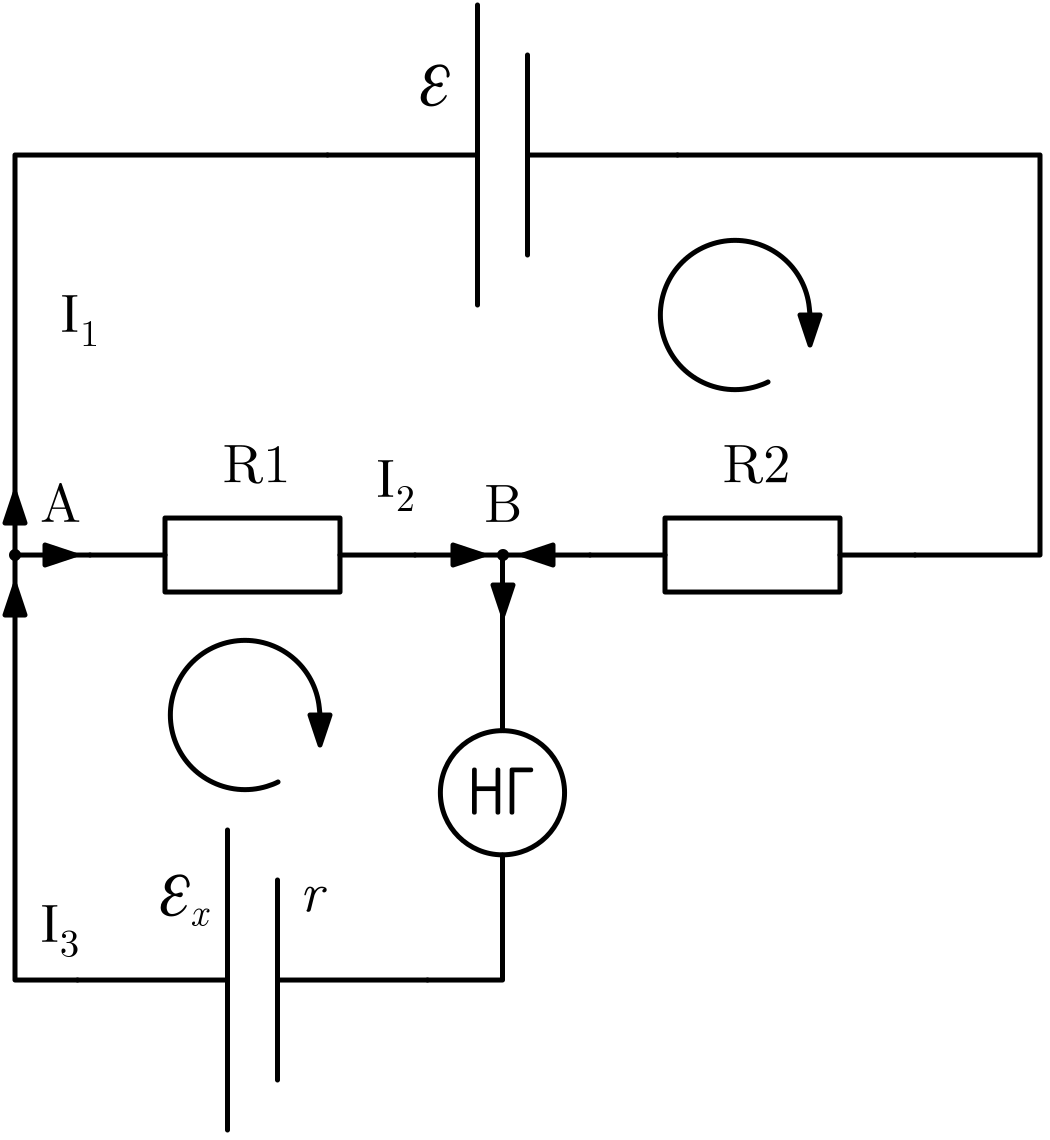
\includegraphics[width=0.5\linewidth]{graph2}
	\caption{Принципиальная схема измерения ЭДС методом компенсации.}
	\label{fig:6}
\end{figure}


\begin{librarybox}
	5. Постройте качественный график зависимости тока через гальванометр от сопротивления $R_1$.
\end{librarybox}

\begin{figure}[H]
	\centering
	\includegraphics[width=\linewidth]{graph5}
	\caption{Качественный график зависимости тока через гальванометр}
	\label{fig:7}
\end{figure}

Значение сопротивления резистора $R_1$ может иметь значения только в диапазоне от $0$ до $R$ из условия \cref{eq:7}. Рассмотрим значения силы тока $I_3$ в этих точках по формуле \cref{eq:8}:
\begin{gather}
	I_3(R) = \frac{R_1\Epsilon - R \Epsilon_x}{rR+R_1R_2} = \frac{\Epsilon - \Epsilon_x}{r}\\
	I_3(0) = -\frac{\Epsilon_x R}{rR} = -\frac{\Epsilon_x}{r}
\end{gather}

Найдем точку пересечения графика с осью абсцисс:
\begin{align}
	0 = \dfrac{R_1 \Epsilon - R \Epsilon_x}{r R + R_1 R_2} \quad\Rightarrow\quad R_1(0) = \frac{\Epsilon_x}{\Epsilon}R
\end{align}

Найдем I и II производные формулы \cref{eq:8} для анализа формы графика:
\begin{multline} \label{eq:4.4}
	I_3' = \left(\frac{R_1 \Epsilon - R_1 \Epsilon_x - R_2 \Epsilon_x}{rR_1 + rR_2 + R_1 R_2}\right)'_{R_1} =\\= \frac{(\Epsilon - \Epsilon_x)(rR_1 + rR_2 + R_1 R_2) - (R_1 \Epsilon - R_1 \Epsilon_x - R_2 \Epsilon_x)(r + R_2)}{\left(rR_1 + rR_2 + R_1 R_2\right)^2} = \\ = \frac{\cancel{rR_1\Epsilon} + rR_2\Epsilon + \cancel{R_1 R_2 \Epsilon} - \cancel{rR_1 \Epsilon_x} - \cancel{rR_2 \Epsilon_x} - \cancel{R_1 R_2 \Epsilon_x}}{(rR_1 + rR_2 + R_1 R_2)^2} -\\- \frac{\cancel{rR_1 \Epsilon_x} - \cancel{rR_1\Epsilon_x} - \cancel{rR_2\Epsilon_x} + \cancel{R_1 R_2 \Epsilon} - \cancel{R_1 R_2 \Epsilon_x} - R_2^2 \Epsilon_x}{(rR_1 + rR_2 + R_1 R_2)^2} = \\ = \boxed{R_2\frac{r \Epsilon + R_2 \Epsilon_x}{(rR + R_1 R_2)^2}} = R_2 (r\Epsilon_x + R_2 \Epsilon_x) (rR_1 + rR_2 + R_1 R_2) ^{-2}
\end{multline}
\begin{multline} \label{eq:4.5}
	I_3'' = \Big(R_2 (r\Epsilon_x + R_2 \Epsilon_x) (rR_1 + rR_2 + R_1 R_2) ^{-2}\Big)'_{R_1} = \\ = -2 R_2 (r\Epsilon + R_2 \Epsilon_x) (r R_1 + r R_2 + R_1 R_2)^{-3} (r+R_2) =\\= \boxed{-2R_2 \frac{(r \Epsilon + R_2 \Epsilon_x)(r + R_2)}{(rR + R_1 R_2)^3}}
\end{multline}




\begin{librarybox}
	6. Как зависит чувствительность компенсационных измерений по схеме на \cref{fig:3} от величины вспомогательной ЭДС $\Epsilon$?
\end{librarybox}

Вспомогательное ЭДС $\Epsilon$ должно быть больше $\Epsilon_x$, для правильного направления тока. Исходя из практических наблюдений $\Delta R_{1x}$ и $\Delta R_{1N}$ уменьшаются с увеличением $\Epsilon$, следовательно, чем выше $\Epsilon$ тем точнее измерение $\Epsilon_x$.

\begin{librarybox}
	7. Как зависит чувствительность компенсационных измерений по схеме на \cref{fig:3} от суммы $R_1 + R_2 = R$?
\end{librarybox}

Для измерения $\Epsilon_x$ нам важно не сумма $R_1 + R_2 = R$, а отношение величины $R_1$ к $R$.